\documentclass[12pt, letterpaper]{article}

\usepackage{spreamble}
\usepackage{graphicx}
\usepackage{tabularx}

\title{CDA3101 - Cache Simulation Project}
\author{Ian Zou}

\begin{document}

\maketitle

\part{Introduction}

To reduce the slowdown of instructions having to access main memory, we use \textbf{cache}. There are a plethora of cache implementations, but the most well known are \textbf{fully associative}, \textbf{direct-mapped}, and \textbf{set associative}.

\section*{Terminology}

\begin{itemize}
    \item \textbf{Fully Associative}: Any cache line may map to any address pointing to main memory.
    \item \textbf{Direct Mapped}: All main memory addresses map to a particular cache line. Multiple addresses may map to the same cache line and cause conflicts.
    \item \textbf{Set Associative}: A middle ground between \textbf{fully associative} and \textbf{direct mapped}. Each main memory address map to a \textbf{set}, which itself is a mini \textbf{fully associative} cache. Conflicts still exist but are mitigated.
    \item \textbf{Cache Size}: The capacity of a particular cache (in bytes).
    \item \textbf{Cache Line Size}: The capacity of a particular cache line (in bytes).
\end{itemize}
\bigskip

For \textbf{fullly associative} and \textbf{set associative} caches, a \textbf{replacement policy} is required to evict addresses from a cache line should the cache reach maximum capacity:

\begin{itemize}
    \item \textbf{Least Recently Used (LRU)}: Keep track of the \textit{least recently used} memory address or \textbf{set} to evict.
    \item \textbf{First In First Out (FIFO)}: Evict the last inserted cache line or from the last inserted \textbf{set}.
\end{itemize}

\section*{Purpose}

\bigskip
The purpose of this \textbf{Cache Simulation Project} is to investigate the relationship between \textbf{cache hit rate} and a cache's \textbf{cache size} and \textbf{block size}. We will also model how different types of caches (\textbf{fully associative}, \textbf{direct mapped}, and \textbf{set associative}) perform comparatively and how \textbf{associative} caches differ in performance when using the \textbf{LRU} replacement policy compared to the \textbf{FIFO} replacement policy.
 
\bigskip

Additionally, we will be taking the \textbf{L1 Caches} of two real-world devices' procesors and running a cache simulation on them, comparing these devices to our testing suite.

\part{Testing Methology}

\section*{Data}

We will be testing every cache type: \textbf{fullly associative}, \textbf{direct mapped}, and \textbf{set associative}. For \textbf{fully associative} and \textbf{set associative} caches, we will also compare the \textbf{LRU} replacement policy to the \textbf{FIFO} replacement policy. For \textbf{set associative} caches specifically, we will be testing the difference between a \textbf{2-way}, \textbf{4-way}, and \textbf{8-way} set associative cache.

\bigskip
We will be creating two \textit{line graphs}: one to illustrate the relationship between \textbf{cache size} vs. \textbf{hit rate}, and another to illustrate the relationship between \textbf{block size} vs. \textbf{hit rate}.

\subsection*{Cache Size vs. Hit Rate}

\begin{itemize}
    \item \textbf{Independent Variable}: Cache Size (bytes) $ \begin{Bmatrix}
            1024 & 2048 & 4096 & 8192 & 16384
    \end{Bmatrix} $
    \item \textbf{Dependent Variable}: Hit Rate (\%)
    \item \textbf{Control Variables}:
        \begin{itemize}
            \item Block Size: $ 64 $ bytes
            \item Trace: \texttt{gcc.trace}
        \end{itemize}
\end{itemize}

\subsection*{Block Size vs. Hit Rate}

\begin{itemize}
    \item \textbf{Independent Variable}: Block Size (bytes) $ \begin{Bmatrix}
            4 & 8 & 16 & 32 & 64
    \end{Bmatrix} $
    \item \textbf{Dependent Variable}: Hit Rate (\%)
    \item \textbf{Control Variables}:
        \begin{itemize}
            \item Cache Size: $ 16384 $ bytes
            \item Trace: \texttt{gcc.trace}
        \end{itemize}
\end{itemize}

\subsection*{Custom Devices}

In addition to the relationships, we will also be plotting two real-world devices against each other. I opted to choose the PS2 (Emotion Engine CPU) and the Nintendo GameCube (Gekko PowerPC CPU) as they similar specifications to the values I had used in the generic test suite and were competing consoles of their generation.

\begin{itemize}
    \item \textbf{Sony PS2 (Emotion Engine)}
        \begin{itemize}
            \item Cache Size: $ 24576 $ bytes (because of limitations of the cache simulator only accepting exponents, we rounded up to $ 2^{15} = 32768 $ bytes)
            \item Block Size: $ 32 $ bytes
        \end{itemize}
    \item \textbf{Nintendo GameCube (Gekko PowerPC CPU)}
        \begin{itemize}
            \item Cache Size: $ 32768 $ bytes
            \item Block Size: $ 32 $ bytes
        \end{itemize}
    \end{itemize}

\section*{Tools}

Professor Resch has generously and graciously provided with us a basic cache simulator written in C++ that takes in arguments from \texttt{stdin} regarding the specifications of a cache, and then a \texttt{.trace} file specifying the memory instructions to simluate on the cache.
\bigskip

However, because of the intense tediousness of inputting every single test individually and then copying those values into an Excel spreadsheet, I sought a slightly more sane solution. Thus, I spent about 5-6 hours overhauling the cache simulator to support generating \texttt{.csv} files with input straight into the code. Running this simulator can be seen in the attached screen recording. Thank goodness I wrote this automator otherwise my sanity may not have been intact :D

\section*{Hypothesis}

\textit{Regarding Correlation:} As the \textbf{cache size}/\textbf{block size} increases, the \textbf{hit rate} will increase.
\bigskip

\textit{LRU vs. FIFO:} \textbf{LRU} should perform better than \textbf{FIFO} on average because its basis on what cache line to evict is based ona ccess and not last inserted, which means that frequently used cache lines will not be dropped and thus increasing the hit rate.

\part{Results}

\begin{figure}[!ht]
    \centering
    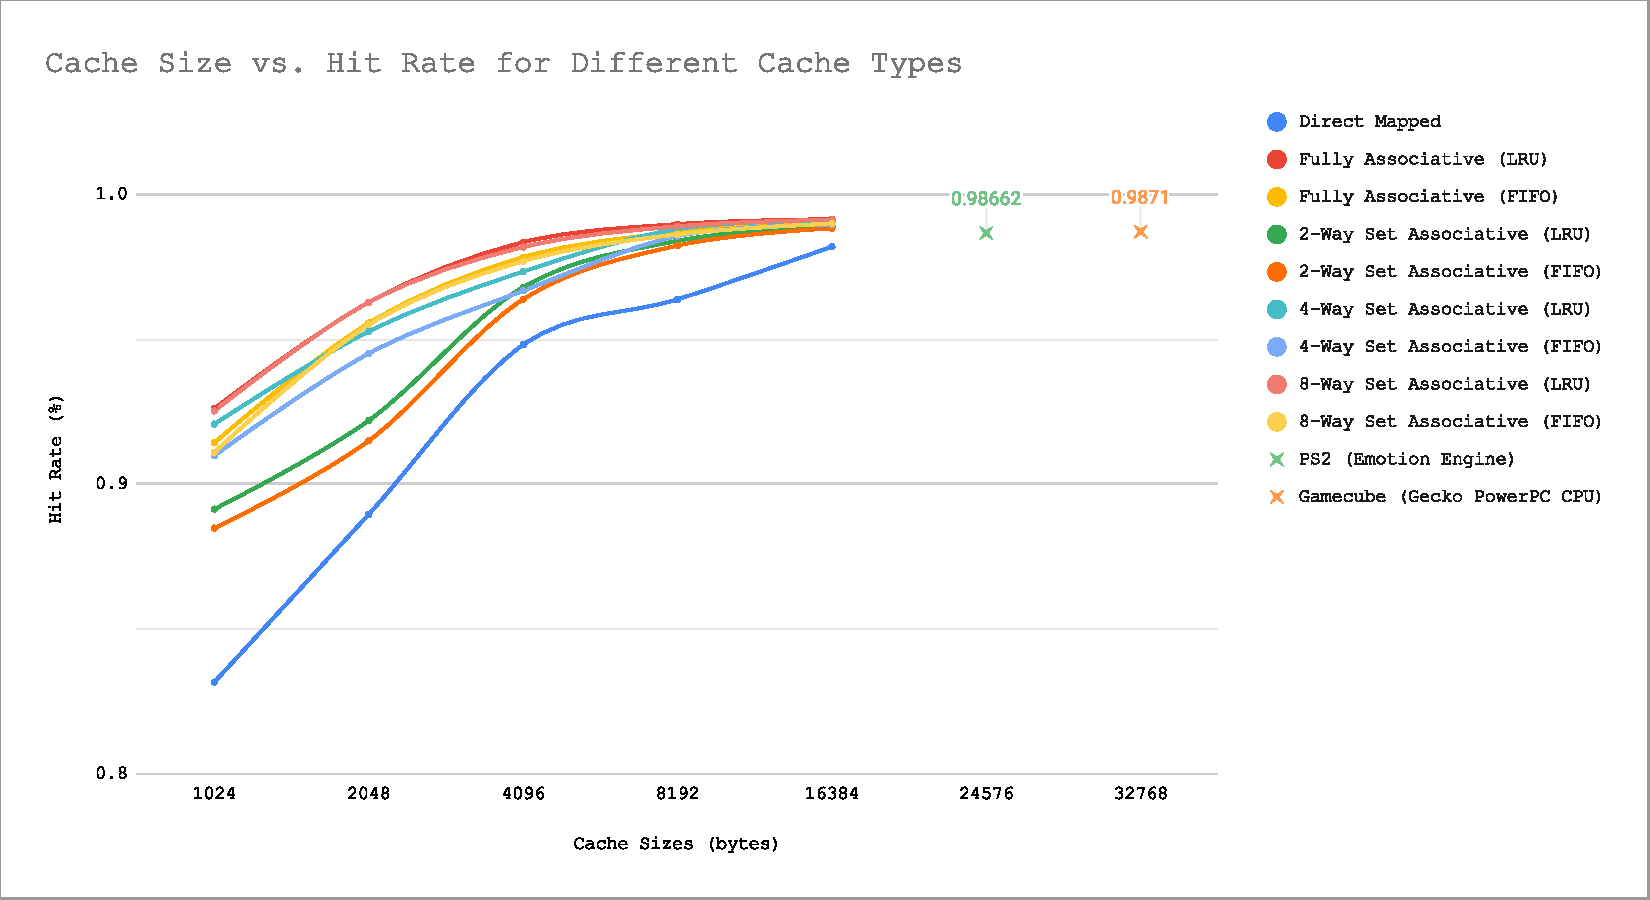
\includegraphics[width=\textwidth]{./cache.pdf}
    \caption{Cache Size vs. Hit Rate for Different Cache Types}
    \label{fig:cache}
\end{figure}
\FloatBarrier

\begin{table}[!ht]
\resizebox{\textwidth}{!}{%
\begin{tabular}{|l|l|l|l|l|l|l|l|l|}
\hline
Cache Sizes                  & 1024    & 2048    & 4096    & 8192    & 16384   & 24576   & 32768  & Averages \\ \hline
Direct Mapped                & 0.83163 & 0.88957 & 0.94803 & 0.96374 & 0.98192 &         &        & 0.922978 \\ \hline
Fully Associative (LRU)      & 0.92603 & 0.96273 & 0.98342 & 0.9897  & 0.9914  &         &        & 0.970656 \\ \hline
Fully Associative (FIFO)     & 0.91424 & 0.95555 & 0.97826 & 0.98691 & 0.99009 &         &        & 0.96501  \\ \hline
2-Way Set Associative (LRU)  & 0.89134 & 0.92193 & 0.96792 & 0.98394 & 0.98922 &         &        & 0.95087  \\ \hline
2-Way Set Associative (FIFO) & 0.88479 & 0.91493 & 0.96372 & 0.9823  & 0.98827 &         &        & 0.946802 \\ \hline
4-Way Set Associative (LRU)  & 0.92069 & 0.95268 & 0.97332 & 0.98801 & 0.99088 &         &        & 0.965116 \\ \hline
4-Way Set Associative (FIFO) & 0.90982 & 0.94505 & 0.96669 & 0.98559 & 0.98953 &         &        & 0.959336 \\ \hline
8-Way Set Associative (LRU)  & 0.92523 & 0.96273 & 0.98178 & 0.98894 & 0.99126 &         &        & 0.969988 \\ \hline
8-Way Set Associative (FIFO) & 0.91095 & 0.95494 & 0.97689 & 0.98616 & 0.98989 &         &        & 0.963766 \\ \hline
PS2 (Emotion Engine)         &         &         &         &         &         & 0.98662 &        &          \\ \hline
GameCube (Gecko PowerPC CPU) &         &         &         &         &         &         & 0.9871 &          \\ \hline
\end{tabular}%
}
\caption{Cache Size vs. Hit Rate for Different Cache Types}
\label{table:cache}
\end{table}
\FloatBarrier

\bigskip
\bigskip
\bigskip

\begin{figure}[!ht]
    \centering
    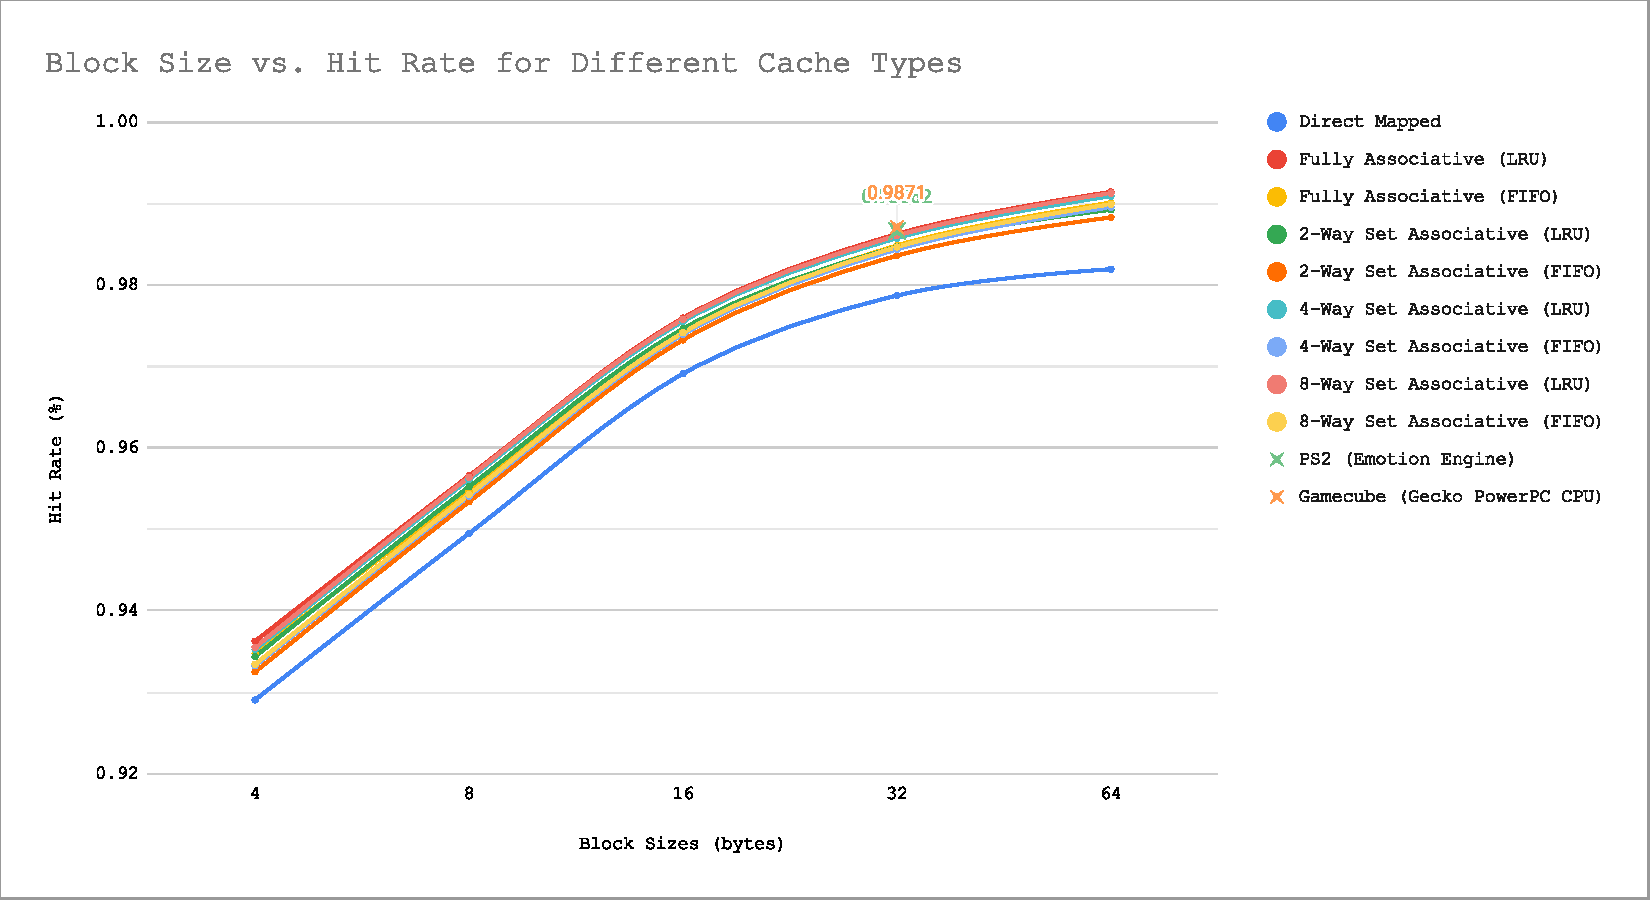
\includegraphics[width=\textwidth]{./block.pdf}
    \caption{Block Size vs. Hit Rate for Different Cache Types}
    \label{fig:block}
\end{figure}
\FloatBarrier

\begin{table}[!ht]
\resizebox{\textwidth}{!}{%
\begin{tabular}{|l|l|l|l|l|l|l|}
\hline
Block Sizes                  & 4       & 8       & 16      & 32      & 64      & Averages \\ \hline
Direct Mapped                & 0.92906 & 0.94949 & 0.96908 & 0.97868 & 0.98192 & 0.961646 \\ \hline
Fully Associative (LRU)      & 0.93627 & 0.95656 & 0.97593 & 0.98624 & 0.9914  & 0.96928  \\ \hline
Fully Associative (FIFO)     & 0.93477 & 0.95469 & 0.9743  & 0.98483 & 0.99009 & 0.967736 \\ \hline
2-Way Set Associative (LRU)  & 0.93437 & 0.95522 & 0.97459 & 0.98466 & 0.98922 & 0.967612 \\ \hline
2-Way Set Associative (FIFO) & 0.93251 & 0.95337 & 0.97323 & 0.98358 & 0.98827 & 0.966192 \\ \hline
4-Way Set Associative (LRU)  & 0.93525 & 0.95611 & 0.9755  & 0.98573 & 0.99088 & 0.968694 \\ \hline
4-Way Set Associative (FIFO) & 0.93324 & 0.95405 & 0.97389 & 0.98435 & 0.98953 & 0.967012 \\ \hline
8-Way Set Associative (LRU)  & 0.93551 & 0.95639 & 0.97577 & 0.98604 & 0.99126 & 0.968994 \\ \hline
8-Way Set Associative (FIFO) & 0.93345 & 0.95426 & 0.97412 & 0.98464 & 0.98989 & 0.967272 \\ \hline
PS2 (Emotion Engine)         &         &         &         & 0.98662 &         &          \\ \hline
GameCube (Gecko PowerPC CPU) &         &         &         & 0.9871  &         &          \\ \hline
\end{tabular}%
}
\caption{Block Size vs. Hit Rate for Different Cache Types}
\label{table:block}
\end{table}
\FloatBarrier

\part*{Conclusion}

As can be observed from \autoref{fig:cache}, the \textbf{hit rate} did indeed correlate with the \textbf{cache size}. As the \textbf{cache size} for all cache types increased, we saw an increase in the \textbf{hit rate}.
\bigskip

Notably, \textbf{direct mapped} was the worst-performing cache type out of the bunch, with an average hit rate of $ 92.298\% $ per \autoref{table:cache}. Interestingly, the \textbf{fully associative w/ LRU} was the best performing ($ 97.066\% $), followed by \textbf{8-way set associative w/ LRU} ($ 96.999\% $). We observe that most associative caches performed better with the \textbf{LRU} replacement policy as opposed to \textbf{FIFO} replacement policy.
\bigskip

We can observe similar findings in \autoref{fig:block}. Our hypothesis regarding \textbf{block size} vs. \textbf{hit rate} also proved to be correct, as it appears that an increasing \textbf{block size} does indeed correlate to an increasing \textbf{hit rate}.
\bigskip

Although the averages are much tighter, \textbf{direct mapped} still appears to perform the worst ($ 95.165\% $) and \textbf{fully associative w/ LRU} still appears to perform the best ($ 96.928\% $), as per \autoref{table:block}. Again, \textbf{LRU} still performs better than \textbf{FIFO} across the board.

\section*{Q\&A}

\begin{itemize}
    \item \textit{Q: How does cache design (direct mapped/set associative/fully associative) affect hit rate?}
        \bigskip

        \textbf{Direct mapped} is the worst performing cache type. This makes sense; \textbf{direct mapped} will cause many conflict misses since many main memory addresses may map to the same cache lines.
        \medskip

        \textbf{Fully associative} appears to be the best performer in terms of hit rate. By design, it has no conflict misses, and coupled with \textbf{LRU}, any frequently used main memory address will rarely be evicted, thus maximizing the chance of cache misses.
        \medskip

        \textbf{Set-associative}, of course, is a good mix of the two. It is widely used as it trades \textbf{hit rate} for the speed of not having to sequentially search every cache line, thus cutting down time (although not measured in our graphs since we only care about hit rate).
    \item \textit{Q: How does hit rate change with the two replacement policies?}
        \bigskip

        The \textbf{LRU} replacement policy is undoubtedly the superior choice. Compared to \textbf{FIFO}, \textbf{LRU} prioritizes whether a memory address has been accessed recently rather than whether the memory address has been inserted recently. If a memory address is accessed often, it should undoubtedly be prioritized within a cache so that repeated accesses are guaranteed a cache hit.
    \item \textit{Q: How does cache size affect hit rate?}
        \bigskip

        \textbf{Cache size} positively correlates to \textbf{hit rate}. As \textbf{cache size} increases, so does \textbf{hit rate}.
    \item \textit{Q: How does line/block size affect hit rate?}
        \bigskip
        
        \textbf{Block size} positively correlates to \textbf{hit rate}. As \textbf{block size} increases, so does \textbf{hit rate}.
    \item \textit{Q: What was the hit rate for the two real devices?  What was the difference in the two devices?  Did one perform better than the other?  What design choices were made?}
        \bigskip

        Because of the limitations of our cache simulator, the severity of the difference in performance of the PS2 to the GameCube is not accurately illustrated, but yes the GameCube does perform better. Not only does it use an \textbf{8-way set associative cache} compared to the PS2's \textbf{2-way set associative cache}, it also should have a significantly greater \textbf{cache size}. Per \hyperref{table:cache}, the hit rate for the PS2 was $ 98.662\% $, whereas the GameCube's hit rate was $ 98.71\% $.
\end{itemize}

\part{Works Cited}

\begin{thebibliography}{4}
    \bibitem{ps2-analysis}
        Rodrigo Copetti, Playstation 2 Architecture, https://www.copetti.org/writings/consoles/playstation-2
    \bibitem{emotion-engine-wikipedia}
        Wikipedia, Emotion Engine, https://en.wikipedia.org/wiki/Emotion\_Engine
    \bibitem{gamecube-wikipedia}
        Wikipedia, GameCube, https://en.wikipedia.org/wiki/GameCube
    \bibitem{gekko-wikipedia}
        Wikipedia, Gekko (Processor), https://en.wikipedia.org/wiki/Gekko\_(processor)

\end{thebibliography}
\end{document}
